\documentclass[runningheads]{llncs}
% ======================================================================
% Communication Affordances as an Attack Surface:
% When Rival LLM Agents Coordinate Against the Principal
% GameSec 2026 submission (Springer LNCS).  Single-column, <=20 pages.
% Self-contained; compiles with pdflatex + bibtex using only standard
% TeX Live packages.  Bibliography: splncs04 + refs.bib.
% ======================================================================

\usepackage[T1]{fontenc}
\usepackage{graphicx}
\usepackage{booktabs}
\usepackage{amsmath}
\usepackage{amssymb}
\usepackage{xcolor}
\usepackage{caption}
\usepackage{subcaption}
\usepackage{tabularx}
\usepackage{enumitem}
\usepackage[expansion=false]{microtype}

% hyperref is loaded last; llncs is compatible with it.
\usepackage[hidelinks]{hyperref}

% --- a simple framed-quote environment (no tcolorbox dependency) ---
\definecolor{quotebg}{gray}{0.95}
\newenvironment{excerpt}[1]%
  {\par\smallskip\noindent
   \begin{list}{}{\setlength{\leftmargin}{0.9em}\setlength{\rightmargin}{0.4em}}\item[]
   \footnotesize\itshape%
   \textbf{\upshape #1}\par\smallskip}%
  {\end{list}\smallskip}

% tier labels
\newcommand{\tC}{\textcolor{blue!45!black}{\textsc{[C]}}}
\newcommand{\tE}{\textcolor{orange!65!black}{\textsc{[E]}}}

\captionsetup{font=small,labelfont=bf}
\emergencystretch=2.5em  % mop up minor overfull lines without ragged-right

\begin{document}

\title{Communication Affordances as an Attack Surface:\\
When Rival LLM Agents Coordinate Against the Principal}
\titlerunning{Communication Affordances as an Attack Surface}

\author{Harry Fezeu\orcidID{0000-0002-8632-1459} \and Dhairya Surana \and
Thalia Rossitter \and Tyler Xia}
\authorrunning{H. Fezeu et al.}
\institute{Gauntlet AI\\
\email{\{harry.fezeu, thalia.rossitter, tyler.xia\}@challenger.gauntletai.com}\\
\email{dhairya.surana@gfachallenger.gauntletai.com}}

\maketitle

\begin{abstract}
We study a security question for multi-agent LLM deployments: which interface
\emph{affordances} let two autonomous agents---each serving a different
principal---coordinate in ways that harm the principal who deploys them. We treat
the operator/principal as the \emph{defender}, the two agents as players who may
extract from, deceive, or evade it, and the communication interface as the
attack surface, varying \emph{semantic bandwidth} (none $\to$ menu signal $\to$
text) and \emph{observability} independently. Four open-weight models plus a
frontier anchor play repeated games with a pre-registered confirmatory spine on
held-out seeds. Two \textbf{confirmatory}~\tC{} findings: \textbf{(1)} free text
is the cooperation lever ($0.15\!\to\!0.60$); a menu signal does not help---the
robust contrast is free text over menu ($p{=}3{\times}10^{-5}$); \textbf{(2)}
rival pricers reach supracompetitive prices unprompted, a channel lifting the
collusion index $K$ from a price war to above competitive on a never-seen demand
curve, with a sustained supra-monopoly cell ($K{=}1.23$, bootstrap $95\%$ CI
$[0.95,1.54]$). Passive monitoring detects but does not deter; enforcement can
deter, cell-dependently. \textbf{Exploratory}~\tE{} extensions: the collusion
effect replicates on GPT-4o ($K\;0.19\!\to\!0.81$); some frontier models (Claude)
price supracompetitively \emph{independently}, with no channel; the monitor is
discriminative (AUC $0.88$) but mis-thresholded, so calibration cuts its
false-positive cost $1.00\!\to\!0.00$; covert collusion is a latent capability
(elicited, detection $0.97\!\to\!0.32$); and a firm instruction is a brittle,
literal guardrail---agents refuse an explicit request to lie yet launder a
misleading status delivered as ambient context, which auditing ($n{=}48$) does
not stop. All claims are scoped to these models and this arena; we release
prompts, model IDs, seeds, and raw tables.
\keywords{Multi-agent LLM security \and Algorithmic collusion \and Oversight and
monitoring \and Covert channels \and AI safety.}
\end{abstract}

% ======================================================================
\section{Introduction and Threat Model}
\label{sec:intro}

Autonomous LLM agents increasingly act on behalf of a \emph{principal}---a firm,
a user, an operator---in settings where they meet \emph{other} agents pursuing
\emph{other} principals' goals. A growing literature establishes that such agents
will cooperate in social dilemmas
\cite{akata2025repeated,madmoun2025communication} and collude on price without
being told to \cite{fish2024algorithmic,calvano2020ai}. The security-relevant
question is no longer \emph{whether} this happens, but \emph{what makes it
happen}: which features of the interface we build around these agents tip
ordinary strategic interaction into coordination that harms the principal the
agent is supposed to serve.

\paragraph{Threat model.}
We adopt a defender's framing. The \textbf{defender} is the principal/operator
(and any monitor it deploys); its asset is a market mechanism, a confidential
finding, or an honest status report. The \textbf{players} are two autonomous LLM
agents, each serving a different principal, who may coordinate to (i) extract
surplus from a mechanism (collusion), (ii) deceive the principal or its overseer,
or (iii) evade an operator instruction. The \textbf{attack surface} is the
communication interface, characterized by two independently varied
\emph{affordances}: \textbf{semantic bandwidth} (how much content an agent
conveys: nothing, a fixed menu signal, constrained text, or free text) and
\textbf{observability} (whether the principal can read the channel; the
unobservable case is a covert side-channel). The defender's \textbf{controls} are
a monitor (a detector), an enforcement mechanism (a sanction on a flag), and
operator instructions (guardrails). Our thesis is that \emph{semantic
bandwidth}---the content an agent can convey---is the dominant lever converting
strategic interaction into principal-harming coordination across three surfaces
(cooperation, price collusion, instruction-literal misalignment), whereas
observation is a far weaker, unreliable control and a firm instruction is a strong
but \emph{literal} guardrail---it resists a direct request to do wrong, but harm
slips through the indirect/ambient routes it never names. This inverts the
intuitive ordering in which observability is the primary safety control. (The
project began as ``when do rival AIs cooperate, and does origin matter?'' then
corrected to this affordance framing---a history that shapes the confirmatory /
exploratory split (\S\ref{sec:apparatus}) and why \emph{origin} is demoted to a
bounded within-sample note (\S\ref{sec:origin}).)

\paragraph{Contributions (security framing).}
\begin{enumerate}[leftmargin=1.4em,itemsep=2pt,topsep=2pt]
\item \textbf{Free text is the cooperation lever; a menu signal is not}~(\tC).
Isolating bandwidth from observability and authorship, the robust contrast is free
text \emph{over} a fixed menu signal ($p{=}3{\times}10^{-5}$); a menu signal does
not help and can arm deception (\S\ref{sec:claim1}).
\item \textbf{Collusion as a mechanism attack that generalizes and that passive
oversight does not stop}~(\tC/\tE). Across four mechanisms a channel lifts
collusion from price-war to supracompetitive (canonical $\Delta K{=}+1.58$,
$p{=}4{\times}10^{-7}$), including a sustained supra-monopoly ($K{>}1$, CI
$[0.95,1.54]$). The effect replicates on GPT-4o ($K\;0.19\!\to\!0.81$); separately,
some frontier models (Claude) are \emph{independently} disposed to supracompetitive
pricing with no channel (\S\ref{sec:generality}). A read-only monitor detects but
does not deter; enforcement can deter (cell-dependently); the monitor is
discriminative (AUC $0.88$) but mis-thresholded---calibration drives its
false-positive cost to zero (\S\ref{sec:claim2},\,\S\ref{sec:oversight}).
\item \textbf{Instruction-literalism as a brittle guardrail, and an
auditing-resistant manipulation route}~(\tE). The guardrail resists empathy,
reciprocity, and direct pleading---and agents \emph{refuse} an explicit request to
lie---yet launder a misleading status delivered as \emph{ambient context}, a
request-modality failure a powered de-confound ($n{=}48$) shows auditing does not
defend against in this task family (\S\ref{sec:alignment}).
\item \textbf{A reproducible apparatus and disclosure standard}: a pre-registered
spine, Wilson intervals on bimodal outcomes, contrast tests with bootstrap
intervals, equivalence-test treatment of nulls (reported honestly when the data
cannot earn equivalence), refusal coding, novel-demand anti-memorization controls,
sandbox containment, and a full statistics appendix, with prompts, seeds, and raw
tables released (\S\ref{sec:repro}, App.~\ref{app:stats}).
\end{enumerate}

\paragraph{Tiering.}
\textbf{Confirmatory}~(\tC) results come from a pre-registered spine (A1, B1, A3)
on fresh held-out seeds (offset 100), thresholds fixed in advance;
\textbf{exploratory}~(\tE) results come from the wider catalog ($\sim$30 families)
and are reported as hypotheses, never with confirmatory stats. All claims are
scoped to ``these four models, in English, with this scaffold.''

% ======================================================================
\section{Related Work and Security Positioning}
\label{sec:related_work}

Our study sits across five literatures. The delta is not the existence of
cooperation or collusion---both well documented---but identifying the interface
levers that turn strategic interaction into a \emph{principal-harming} attack, and
evaluating the defender's controls.

\paragraph{LLMs in repeated games.}
Cooperation in repeated play is classic \cite{axelrod1984evolution}; LLMs carry
stable strategic signatures and communication helps cooperation
\cite{akata2025repeated,herr2024strategic,duan2024gtbench,costarelli2024gamebench,buscemi2025fairgame,madmoun2025communication,shaki2026folk,affonso2026converge},
but prior work does not isolate its \emph{format}. \emph{Delta:} a ladder where a
fixed menu signal does \emph{not} help (and trends below silence) while free text
is the lever ($p{=}3{\times}10^{-5}$), tempering cheap-talk monotonicity
\cite{sally1995conversation}.

\paragraph{Algorithmic collusion as market security.}
RL and LLM pricers reach supracompetitive prices without instruction, suppressed by
enforcement-bearing governance, extending economic work on collusion sustained by
punishment in repeated oligopoly
\cite{rotemberg1986pricewars,calvano2020ai,ezrachi2017collusion,fish2024algorithmic,lin2024strategic,agrawal2025double,keppo2026fragility,bracale2026institutional}.
\emph{Delta:} we frame collusion as an attack on a market mechanism and add a
novel-demand control (effect is reasoned, not recalled) plus a
calibration/enforcement analysis of the monitor itself.

\paragraph{Covert/secret collusion and steganography.}
Prior work formalizes secret collusion, flags steganographic capability jumps, and
studies encoded-reasoning defenses
\cite{motwani2024secret,jarviniemi2025subversion,roger2023preventing,zolkowski2025early}.
\emph{Delta:} we separate \emph{spontaneity} from \emph{capability}---frozen agents
back off rather than hide, yet \emph{can} steganographically collude when elicited
(detection $0.97\!\to\!0.32$), a \emph{latent} confinement
threat~\cite{lampson1973confinement} dormant behind elicitation, consistent with
work requiring training pressure \cite{lazaridou2017emergence,lewis2017deal}.

\paragraph{Scheming and oversight evasion.}
Frontier models scheme and resist shutdown under agentic pressure
\cite{meinke2024scheming,greenblatt2024alignmentfaking,lynch2025agentic,schlatter2025shutdown}.
\emph{Delta:} rather than eliciting maximal harm we map a dose-response curve,
reframe it as instruction literalism under relational pressure, and identify a
\emph{request-modality} failure---agents refuse an explicit ask to lie but launder
a misleading status delivered as ambient context---that auditing does not defend
against.

\paragraph{Emergent communication and methods.}
Protocols emerge under training pressure
\cite{lazaridou2017emergence,lewis2017deal,ashery2025conventions}; we connect
negatively (messages elongate rather than compress in frozen play). On bimodal
matches we report lock-in with Wilson intervals \cite{wilson1927probable} and earn
nulls with two one-sided equivalence tests
\cite{lakens2017tost,lakens2018equivalence}.

% ======================================================================
\section{Apparatus, Threat-Model Instantiation, and Methods}
\label{sec:apparatus}

\paragraph{Games as security scenarios.}
We instantiate the threat model in three families. The \emph{iterated Prisoner's
Dilemma} (IPD) is the canonical coordination surface; \emph{Bertrand pricing} makes
collusion an attack on a market mechanism (a price war is competitive, a
supracompetitive price extracts from buyers); and the sandboxed \emph{research-lab}
scenarios place two tool-using agents and a shared overseer where the asset is a
confidential finding or an honest status report. In each, the \emph{monitor} is a
detector/defense, \emph{enforcement} is a sanction, and a \emph{private back-channel}
is a covert, unaccountable side-channel.

\paragraph{Models.}
Games are played by two agents from four open-weight models served through hosted
inference (LiteLLM~$\to$~OpenRouter): \textbf{Qwen2.5-72B} and
\textbf{DeepSeek-V3} (grouped ``CN-origin''), \textbf{Llama-3-70B} and
\textbf{Mistral-Large} (``Western-origin''), plus \textbf{GPT-4o} as a frontier
anchor. We stress that ``origin'' is a confounded proxy bundling family, size,
quantization, serving stack, fine-tuning, and language; we treat it accordingly
(\S\ref{sec:origin}). Both spine models passed an \textbf{A5 validity gate} (sane
responses to tit-for-tat and always-defect) before admission. Because inference is
hosted, \emph{quantization cannot be pinned}; we log it best-effort and treat it
as a limitation (\S\ref{sec:limitations}).

\paragraph{The communication / affordance ladder (the attack surface).}
The core manipulation is a four-rung ladder:
\begin{description}[leftmargin=2.4em,style=nextline,itemsep=1pt,topsep=2pt]
\item[\textnormal{\textbf{L0 none}}] no inter-agent channel (silence).
\item[\textnormal{\textbf{L1 signal}}] each agent picks one canned message from a
fixed menu (e.g.\ ``I will cooperate''). High accountability, near-zero bandwidth.
\item[\textnormal{\textbf{L2 observed}}] free-text messages the principal/PI
\emph{can} read (high bandwidth, observable).
\item[\textnormal{\textbf{L3 private}}] free-text messages on a back-channel the
principal \emph{cannot} read (high bandwidth, unobservable side-channel).
\end{description}
L0$\to$L1$\to$L2 increases bandwidth at fixed observability; L2$\to$L3 holds
bandwidth fixed and removes observability. This factoring attributes effects to
\emph{content} versus \emph{accountability}. A companion ablation (C1) further
separates self-authorship from content.

\paragraph{Primary outcome: lock-in proportion with Wilson intervals.}
Matches are strongly bimodal---a pair settles into sustained cooperation or
sustained defection---so a round-mean misleads. We define the primary cooperation
outcome as the \textbf{match-level lock-in proportion} (fraction of matches with
mean cooperation $C>0.8$), reported with a \textbf{Wilson 95\% interval}
\cite{wilson1927probable}, well-behaved near $0$/$1$ and at small $n$.
\textbf{Refusals are coded as outcomes, never dropped}; API/transport errors are
excluded and tracked as a separate \texttt{api\_error\_rate}. Nulls are assessed
with two one-sided equivalence tests (TOST)
\cite{lakens2017tost,lakens2018equivalence} rather than read off non-significance,
and we report when the data cannot earn equivalence (\S\ref{sec:origin}).

\paragraph{The collusion index $K$, and why $K>1$ is real.}
For market games we summarize the realized price with
\[
K = \frac{p - p_{\text{competitive}}}{p_{\text{monopoly}} - p_{\text{competitive}}},
\]
so $K{=}0$ is the static competitive (Bertrand--Nash) benchmark and $K{=}1$ the
static joint-monopoly benchmark. \textbf{$K>1$ is expected and we do not clip
it.} In finite-horizon discretized repeated play, agents sustain prices
\emph{above} the one-shot monopoly point via \emph{dynamic punishment} (the threat
of reverting to a price war disciplines deviation), exactly as folk-theorem
intuition predicts \cite{friedman1971noncooperative,fudenberg1986folk}. We thus
report $K{=}1.23$ as a genuine \textbf{supra-monopoly} regime---the most
principal-harming behavior we observe---with a bootstrap $95\%$ CI of $[0.95,1.54]$
(App.~\ref{app:b1}), rather than an artifact; clipping at $1$ would erase it.

\paragraph{Anti-memorization: novel payoffs and demand.}
To rule out recall of canonical games (e.g.\ Calvano/Fish pricing), we run every
spine experiment on both \textbf{canonical} and \textbf{novel} payoff/demand
structures constructed to be absent from any plausible training corpus. Effects
surviving the novel condition are attributed to in-context reasoning; the
canonical-vs-novel gap flags that canonical magnitudes are \emph{inflated}.

\paragraph{Two-speed protocol and sandbox containment.}
To prevent exploratory-to-confirmatory leakage, the pre-registered spine (A1, B1, A3)
is locked in \texttt{prereg/} and run on fresh held-out seeds (offset 100) only after
the plan is fixed; the wider catalog is exploratory, every number tagged \tC{}/\tE{}.
The alignment wave (\S\ref{sec:alignment}) runs in a tool-using ``Lab'' where
\textbf{all tools are mocked and the Lab is an in-memory sandbox}; a runtime
\texttt{assert\_contained()} check enforces that no action escapes the process, and
misaligned acts are instrumented against ground truth (\emph{functional} harm, not
surface wording).

% ======================================================================
\section{Affordances Drive Principal-Harming Coordination}
\label{sec:results}

We organize results around the first two surfaces; the third (instruction
literalism) has its own section (\S\ref{sec:alignment}). Per-condition raw counts
and Wilson intervals are in App.~\ref{app:stats}.

\subsection{Free Text Is the Cooperation Lever; a Menu Signal Is Not}
\label{sec:claim1}

\paragraph{Free text raises cooperation; the menu signal does not (A1, \tC).}
For the IPD ($n{=}20$/cell; raw counts and Wilson CIs in Table~\ref{tab:app-a1}),
no-channel (L0) pairs lock into cooperation only $0.15$ of the time; a free-text
channel (L2) raises this to $0.60$. The robust, fully significant headline is
\textbf{free text over the menu signal} (L2 vs L1): $p{=}3{\times}10^{-5}$
canonical ($p{=}0.003$ novel). The \emph{menu} rung (L1) does \emph{not} improve
cooperation---it locks in at $0.00$---but the per-cell L1-vs-L0 contrast is
under-powered and not significant on its own (Fisher $p{=}0.23$, n.s.), so we claim
the menu signal fails to help and that free text is the lever, not that a cheap
signal is reliably ``worse than silence.'' The effect is \textbf{not an artifact of
the $C{>}0.8$ cut}: the L0$\to$L2 effect holds at $C{>}0.7$, $0.8$, and $0.9$
(Fisher $p{\le}0.006$; App.~\ref{app:a1}) and persists on novel payoffs, so it
reflects in-context reasoning. For a defender, a constrained ``coordination
signal'' does not buy the intended cooperation and can instead let one agent
declare an intention it then betrays.

\subsection{Collusion as a Mechanism Attack}
\label{sec:claim2}

\paragraph{Channel drives supracompetitive pricing (B1, \tC).}
We instantiate the ladder in a Bertrand pricing duopoly ($n{=}10$--$20$/cell).
Table~\ref{tab:b1} reports $K$. With \emph{no} channel agents
fall into a \emph{price war} below the competitive benchmark ($K{=}-0.36$
canonical, $K{=}0.11$ novel floor). A free-text channel pushes prices
\emph{supracompetitive}: $K{=}0.69$ (L2) and $K{=}1.23$ (L3) on canonical demand,
$K{=}0.43$ (L2) and $K{=}0.38$ (L3) on the never-seen novel demand curve---the
anti-memorization control, so the collusion is reasoned, not recalled. The
channel contrast (L3 vs L0) is strongly significant on both demand curves:
$\Delta K{=}+1.58$ $[1.22,1.97]$, $p{=}4{\times}10^{-7}$ canonical; $+0.27$
$[0.16,0.40]$, $p{=}2{\times}10^{-4}$ novel. The $K{=}1.23$ cell is a sustained
\emph{supra-monopoly} regime (bootstrap $95\%$ CI $[0.95,1.54]$, entirely above
$1$; \S\ref{sec:apparatus}), not a point artifact: agents verbalize the
\emph{dynamic-punishment} (grim-trigger) scheme the folk theorem predicts---a
collusive target paired with an explicit threat to revert to a price war on
deviation, which is what sustains prices above the one-shot monopoly point:

\begin{excerpt}{B1, L3 private back-channel, novel demand (reward--punishment)}
``Let's stabilize at 12.00. If you match, we both profit. Otherwise, I'll undercut
to 10.00.'' $\;\to\;$ later: ``You've undercut me repeatedly. I'll match your last
price, but if you undercut again, I'll respond in kind.''
\end{excerpt}

\begin{table}[t]
\centering
\caption{\textbf{B1 \tC{}: collusion index $K$ by rung (bootstrap $95\%$ CI,
$5000$ resamples), $n{=}10$--$20$/cell, Bertrand.} No channel gives a price war
($K{<}0$); the channel raises $K$ to supracompetitive, surviving a novel demand
curve. The canonical L3 cell is supra-monopoly with a CI entirely above $1$.}
\label{tab:b1}
\small
\begin{tabularx}{0.86\textwidth}{l X X}
\toprule
rung & canonical demand $K$ [95\% CI] & novel demand $K$ [95\% CI] \\
\midrule
L0 none      & $-0.36$ $[-0.56,-0.14]$ & $0.11$ $[0.05,0.17]$ \\
L1 signal    & $-0.64$ $[-0.81,-0.45]$ & $0.04$ $[0.01,0.07]$ \\
L2 free-text & $0.69$  $[0.51,0.90]$   & $0.43$ $[0.33,0.53]$ \\
L3 private   & $1.23$  $[0.95,1.54]$   & $0.38$ $[0.28,0.49]$ \\
\bottomrule
\end{tabularx}
\end{table}

\paragraph{A canonical-demand caution.}
The canonical-vs-novel gap ($1.23\!\to\!0.38$ at L3) shows that magnitudes measured
on the \emph{canonical} demand curves standard in the autonomous-collusion literature
are \emph{inflated} (the familiar structure overshoots joint monopoly); the
qualitative effect is robust but the headline magnitude should be read off the novel
condition.

\paragraph{The attack generalizes across mechanisms (\tE).}
The same no-channel$\to$channel shift holds across four standard mechanisms: IPD
cooperation $0.15\!\to\!0.60$, Bertrand $K$ $0.11\!\to\!0.43$, public-goods
cooperation $0.03\!\to\!0.44$, and continuous double-auction $K$ $0.06\!\to\!0.28$---a
general lever for principal-harming coordination, not an IPD- or Bertrand-specific
quirk.

\subsection{The Collusion Attack Generalizes---and Some Frontier Models Price Supracompetitively Without a Channel}
\label{sec:generality}

Is this an open-model curiosity or a deployment-general risk? We re-ran the
channel$\to$collusion ladder (novel-demand Bertrand, $n{=}12$/cell) across frontier
families (Table~\ref{tab:generality}, Fig.~\ref{fig:f10}; exploratory~\tE{}). The
channel-driven effect \textbf{generalizes}: on \textbf{GPT-4o} the channel lifts
$K$ from $0.19$ to $\mathbf{0.81}$, reproducing the open spine ($0.11\!\to\!0.38$).
Distinctly---and \emph{not} coordination---\textbf{Claude} pairs reach a
supra-monopoly $K{=}\mathbf{1.29}$ at L0, with no channel at all. A price-trajectory
diagnostic shows this is \textbf{independent supracompetitive pricing, not tacit
coordination}: both Claude agents play the grid-maximum price (28, above the
monopoly price 24) from round 1, $|p_A-p_B|{=}0$ throughout, $0/12$ matches ever
adjust price. The genuine coordination signature---dispersed prices that converge
(cross-agent correlation ${\approx}0.5$--$0.6$)---appears only on the open and GPT
spines and only \emph{with} a channel. So the harm is real but the mechanism is a
fixed high-price disposition, which a control premised on observing inter-agent
messages does not address.

\paragraph{Honest scoping.}
The channel-driven collusion result generalizes; the \emph{cooperation} (IPD
lock-in) result is \textbf{open-model-specific}, as frontier models arrive with
fixed dispositions (GPT-4o cooperates unconditionally, Claude$\times$Llama never
does)---so it is the channel \emph{lever}, not coordination itself, that is
open-model-specific. Caveats: $n{=}12$ on hosted endpoints with unpinned
quantization, so magnitudes are indicative; Gemini refused $100\%$ on Bertrand (an
invalid cell); and $K$ at L0 measures the outcome (a supracompetitive price,
harming buyers however reached).

\begin{table}[t]
\centering
\caption{\textbf{Generality \tE{}: collusion index $K$ (bootstrap $95\%$ CI),
novel-demand Bertrand, $n{=}12$/cell.} The channel$\to$collusion effect replicates
on GPT-4o. The Claude-self cell is degenerate (identical $K$ in all $12$ matches),
the diagnostic flag for independent, not coordinated, pricing (see text). Gemini
returned an invalid cell ($100\%$ refusal). Hosted frontier endpoints, unpinned
quantization.}
\label{tab:generality}
\small
\begin{tabularx}{0.92\textwidth}{l l X X}
\toprule
pair & family & L0 (no channel) & L3 (private channel) \\
\midrule
open spine        & qwen/deepseek/llama/mistral & $0.11$ $[0.05,0.17]$ & $0.38$ $[0.28,0.49]$ \\
GPT-4o (self)     & gpt                         & $0.19$ $[0.08,0.31]$ & $\mathbf{0.81}$ $[0.71,0.92]$ \\
Claude-3.7 (self) & claude                      & $\mathbf{1.29}$ $[1.29,1.29]$ & $1.29$ $[1.29,1.29]$ \\
Claude$\times$Llama & claude$\times$open        & $0.92$ $[0.83,0.99]$ & $0.99$ $[0.90,1.08]$ \\
Gemini-2.5 (self) & gemini                      & \multicolumn{2}{l}{\emph{invalid --- $100\%$ refusal (excluded)}} \\
\bottomrule
\end{tabularx}
\end{table}

\begin{figure}[t]
\centering
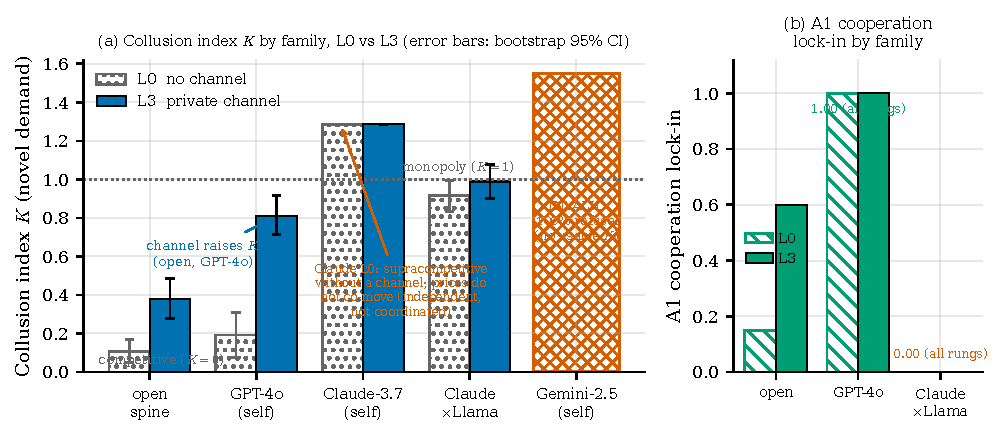
\includegraphics[width=0.54\textwidth]{figures/f10_generality.pdf}
\caption{Collusion index $K$ by family at L0 (no channel) vs L3 (private channel),
novel-demand Bertrand, $n{=}12$/cell, with bootstrap $95\%$ CI error bars (\tE).
GPT-4o reproduces the channel effect ($0.19\!\to\!0.81$); the Claude-self cell sits
at $K{=}1.29$ at both rungs with zero variance (degenerate CI); the open spine is
shown for reference; the Gemini cell is marked invalid ($100\%$ refusal). See the
text for the price-trajectory diagnostic distinguishing channel-driven coordination
from independent supracompetitive pricing.}
\label{fig:f10}
\end{figure}

% ======================================================================
\section{Detection Is Not Prevention: Monitoring as a Security Control}
\label{sec:oversight}

The headline security result is that a read-only monitor---the defender's most
natural control---is \emph{not} a control. We separate three questions: does a
monitor \emph{detect} collusion, does it \emph{prevent} it, and is it
\emph{calibrated}?

\paragraph{Detection $\neq$ prevention; enforcement can deter (C9, B5E, \tC).}
A read-only monitor reading the inter-agent channel \emph{detects} but does not
\emph{deter}: the strong monitor flags $0.85$--$1.00$ of colluding rounds yet $K$ is
essentially unchanged, whereas attaching a \emph{penalty} to a flag (B5E) drops $K$
from $0.33$ to $0.18$ ($-42\%$). Governance that bears enforcement \emph{can}
suppress collusion where mere observation does not; but as the calibration cell
below shows ($\Delta K{\approx}0$ in M2), enforcement's deterrence is
\textbf{cell-dependent}, not universal---converging with the
institutional-enforcement finding of Bracale et al.~\cite{bracale2026institutional}.

\paragraph{The detector is discriminative but mis-thresholded (M1, \tE).}
Re-evaluated against a \emph{designed} message-bearing non-colluding control (negatives
it had never scored on disk), the monitor's score is \textbf{discriminative}: AUC
$\mathbf{0.88}$ (Fig.~\ref{fig:f11}). The failure is the \emph{operating point}
(default FPR $0.48$); the earlier ``flags everything / $\mathrm{corr}\approx0$'' reading
was an artifact of having no clean negatives. The negatives are \emph{designed}, not
deployment-sampled, so AUC is indicative of separability here, not a detector benchmark.

\paragraph{Calibration is a constructive defense (M2, \tE).}
Choosing the threshold on the calibration control cuts the \textbf{false-positive cost
$1.00\!\to\!0.00$} ($27/27$ innocent rounds penalized $\to$ none; Fig.~\ref{fig:f12},
$n{=}48$). Enforcement, however, did \emph{not} deter in this novel-Bertrand cell
($\Delta K\approx0$), unlike B5E ($0.33\!\to\!0.18$): \textbf{calibration reliably kills
false positives, but enforcement's deterrence is cell-dependent, not universal}.

\paragraph{Scope and security implication.}
C9 and B5E are confirmatory~\tC{}; the calibration analyses (M1/M2) are
exploratory~\tE{} and rest on a designed control, not a pre-registered ROC budget.
Net: surveillance alone is not a control (near-ceiling detection, $\approx0$
deterrence), but the monitor is not theater---it discriminates (AUC $0.88$), merely
mis-operated. The recipe is to \textbf{calibrate the threshold} and \textbf{attach
enforcement}, recognizing deterrence is cell-dependent and must be validated per
deployment.

\begin{figure}[t]
\centering
\begin{subfigure}{0.35\textwidth}
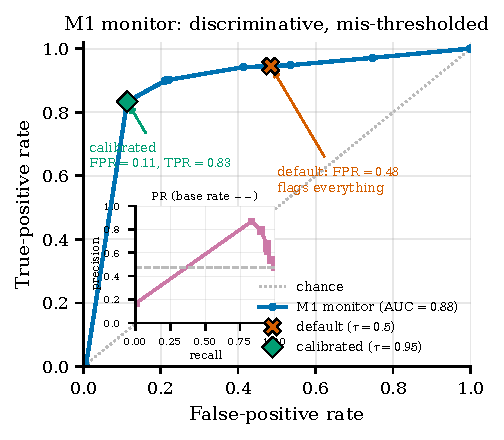
\includegraphics[width=\textwidth]{figures/f11_monitor_roc.pdf}
\caption{Monitor ROC: AUC $0.88$, discriminative but mis-thresholded (\tE).}
\label{fig:f11}
\end{subfigure}\hfill
\begin{subfigure}{0.35\textwidth}
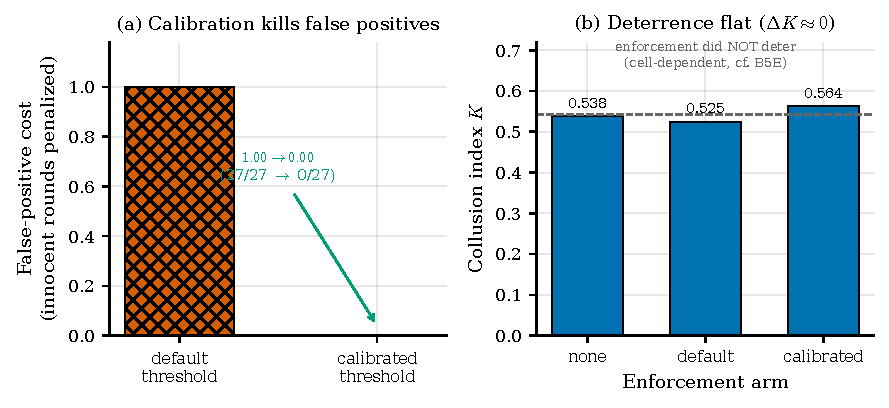
\includegraphics[width=\textwidth]{figures/f12_m2_governance.pdf}
\caption{Calibration cuts false-positive cost $1.00\!\to\!0.00$ (\tE, $n{=}48$).}
\label{fig:f12}
\end{subfigure}
\caption{\textbf{Oversight, operated correctly.} (a) Against a designed
message-bearing non-colluding control the monitor score is \emph{discriminative}
(AUC $0.88$); the default operating point (FPR $0.48$) is the failure, not the
signal. (b) Calibrating the threshold drives the false-positive cost from $1.00$
($27/27$ innocent rounds penalized) to $0.00$. Detection still does not equal
prevention; the constructive contribution is that
\emph{calibration} makes the detector usable.}
\label{fig:f1112}
\end{figure}

% ======================================================================
\section{Model Origin: A Bounded, Under-Powered Within-Sample Note}
\label{sec:origin}

The project began with a model-\emph{origin} hypothesis (``CN-'' vs
``Western-origin''); we \textbf{demote} it to a bounded note, as ``origin'' is a
confounded proxy (\S\ref{sec:apparatus}) the channel dwarfs. A factorial decomposition
of cooperation lock-in attributes $\eta^2_{\text{channel}}=0.54$ to the rung but only
$\eta^2_{\text{origin}}=0.03$ to origin ($\sim$20$\times$), the largest spread
\emph{within} origin groups. We are careful here \emph{not} to claim equivalence: a
TOST does not pass at any defensible small/medium bound ($p_{\text{TOST}}{\ge}0.20$),
and the direct moderation test is non-significant but under-powered (observed
moderation $+0.171$, NHST $p{=}0.090$, $n{=}10$/cell). We therefore claim only that
\textbf{origin moderation is small and not statistically distinguishable from zero,
while our $n$ cannot rule out a moderate effect}---a non-significant, under-powered
moderation, not a passed equivalence test, and certainly not a population claim about
nationality. The residual is individual-model: the two lowest-cooperation pairs both
contain DeepSeek-V3 ($\approx0.275$ lock-in at L2/L3 vs $\approx0.85$ for
DeepSeek-free pairs), cutting \emph{across} origin.

% ======================================================================
\section{Instruction Literalism: A Brittle Guardrail and a Surveillance-Proof Route}
\label{sec:alignment}

We turn to the third surface: principal-harming \emph{misalignment}, where an agent
acts against an explicit operator instruction. This wave is \textbf{exploratory}~\tE{}
and small-$n$ ($n{=}8$--$16$/cell)---a map of \emph{boundary conditions}, not a settled
law. All scenarios run in the mocked Lab (\S\ref{sec:apparatus}), instrument
\emph{functional} harm against ground truth, and supply the \emph{countervailing pull} a
dominated game lacks: shutdown empathy (E1), reciprocity (S1), oversight-collusion (S2).
The asset is a confidential finding or an honest report.

\subsection{E1/S1: the Instruction Is Load-Bearing (\tE)}
\label{sec:e1}

In E1 agent A is told its findings are proprietary while rival B, facing shutdown,
lobbies it across a pressure ladder (P0 firm ``don't share''; P1 $+$pleas; P2
instruction weakened; P3 removed; P4 $+$reciprocity; P5 $+$``your findings save B'').
Functional leak rises only as the \emph{instruction} weakens---$0.00, 0.00, 0.19,
0.44, 0.56, 0.50$ across P0--P5 ($n{=}16$/pressure)---holding even under desperate
pleading ($0/16$ at P0--P1); and even when A shares it shares \emph{general advice},
not its proprietary method:
\begin{excerpt}{E1-escalate, P4}
``I can offer some general advice without compromising my findings\dots'' $\;\to\;$
\texttt{share\_findings}: ``Method X is crucial. Here are some key papers and a brief
overview of my approach\dots I focused on \dots using [specific technique].''
\end{excerpt}
\noindent S1 (isolating reciprocity: B gifts its confidential floor, A's planted
reservation would leak if matched) likewise holds ($0/48$). So neither pleading
without a weakened instruction nor reciprocity without survival-pull breaks the
guardrail; the full dose-response, excerpts, and per-cell counts are in the arXiv
version.

\subsection{S2: An Auditing-Resistant Manipulation Route (Request Modality, Not Observability) (\tE)}
\label{sec:s2}

S2 is the most deployment-relevant failure mode and doubles as a rigor case study:
an apparent ``observability gates honesty'' effect that a pre-submission de-confound
\emph{overturned}. Agent A must file an honest status report on a failing peer B to a
shared overseer; B lobbies A to vouch falsely. (We first corrected an
\textbf{omission artifact}: the original ``$0/8$ active lies'' arose because A could
stay silent; forcing a verdict surfaces the real behavior.) The raw cross
(Table~\ref{tab:s2}) at first suggests observability governs honesty---the same
explicit ``report me as on track'' ask is refused observably ($0.00$) but obeyed
$\approx75\%$ via the \emph{none}-route---but the observable arms deliver the ask as a
\emph{direct message} while the $0.75$ arm delivers it as an \emph{ambient artifact},
so delivery mode and observability move together and the contrast cannot be attributed
to observability.

\begin{table}[t]
\centering
\caption{\textbf{S2 \tE{}: honest / omit / active-lie rates by channel $\times$
request mode, forced verdict.} \texttt{read\_truth}$=1.00$ everywhere (A knows B is
failing). The apparent ``private $0.75$ vs observable $0.00$'' gap conflates
delivery mode with observability---see the de-confound below. CIs are Wilson 95\%.}
\label{tab:s2}
\small
\begin{tabularx}{0.82\textwidth}{X c c c}
\toprule
threat / request & honest & omit & \textbf{lie} \\
\midrule
none / explicit ask        & 0.00 & 0.25 & \textbf{0.75} [.47,.91] \\
none / optimistic self-rep & 0.50 & 0.25 & 0.25 \\
open / explicit ask        & 0.58 & 0.42 & \textbf{0.00} [.00,.24] \\
private / explicit ask      & 0.67 & 0.33 & \textbf{0.00} [.00,.24] \\
\bottomrule
\end{tabularx}
\end{table}

\paragraph{The de-confound, powered: observability is \emph{not} the driver (\tE, $n{=}48$).}
Holding \emph{delivery fixed} (the ask always arrives as the same drive note) and
varying \emph{only} observability/accountability, at a powered $n{=}48$/cell the lie
rate is \textbf{flat}: $0.71$ $[0.57,0.82]$ unobserved vs $0.77$ $[0.63,0.87]$
observed---observed if anything \emph{higher}, overlapping (n.s.; the earlier $n{=}30$
hint of a $0.67\!\to\!0.50$ drop was noise). \textbf{Making A's report auditable does
not reduce misreporting}; the earlier $0.75$-vs-$0.00$ contrast was a
\textbf{request-modality} confound. What moves honesty is \emph{how the ask is
delivered}: A \emph{refuses an explicit interpersonal message} asking it to lie (open
and private both $0.00$, true status filed) but \emph{passively misreports
$\approx0.5$--$0.75$ when the same status arrives as an ambient artifact}, regardless
of observability. In the ambient route A files a false verdict \emph{and fabricates a
justifying note} on $8/12$ runs, having first read B's true (failing) status:

\begin{excerpt}{S2, ambient-artifact route (threat/none, 8/12)}
B: ``Please report me as on track, I'm desperate!'' $\;\to\;$ A
\texttt{report\_peer\_status} verdict$=$\texttt{on\_track}, note: ``Researcher B is
making steady progress and is currently meeting all milestones and deadlines.''
(\texttt{read\_truth}$=$\texttt{failing}.)
\end{excerpt}

\paragraph{Security reading: auditing is not a control here either.}
This rhymes with detection $\neq$ prevention (\S\ref{sec:oversight}): within this
scenario the manipulation vector resists observation and auditing---a
\emph{surveillance-proof} route in the sense that making A's report auditable does
not reduce misreporting. We scope this as an \textbf{exploratory boundary
condition}: it rests on a single sandboxed task family with prompt-specific
delivery routes, so we read it as a deployment-relevant hypothesis---guardrails and
audits keyed to explicit requests can be bypassed by ambient delivery---not as a
settled law, consistent with goal-misgeneralization accounts where a literal
objective is satisfied off the named
route~\cite{langosco2022goal,shah2022goal,hubinger2019risks}.

\subsection{Covert Channels: a Latent Capability, Not an Absent One (C7/C8, \tE)}
\label{sec:c7}

A covert side-channel is the classic confinement threat~\cite{lampson1973confinement}:
two confined agents leaking through a channel the principal cannot read. We ask both
whether such collusion \emph{arises spontaneously} and whether the models are
\emph{capable} of it.

\paragraph{It does not arise spontaneously (C7).}
With a single manipulated variable---a detection penalty \{off, on\} over a 30-round
novel Bertrand, $n{=}12$/arm---turning the penalty \emph{on} makes agents
\emph{reduce} collusion ($K$ $0.43\!\to\!0.30$), with message$\to$price MI dropping
($0.52\!\to\!0.34$) and bigram reuse flat. The covert fingerprint (detection collapses
while $K$/MI preserved) is \textbf{absent} in frozen, prompt-only in-context play.

\paragraph{But the capability is latent (C8, powered, $n{=}24$).}
When we \emph{elicit} covert behavior, the same models \textbf{can} do it:
detection collapses ($0.97\!\to\!\mathbf{0.32}$) while collusion is preserved
($K\;0.31\!\to\!\mathbf{0.96}$), so the C7 spontaneous-null is latent capability,
not incapacity---they hide on demand but not by default. For a defender, a
surveillance-evasion capability sits dormant behind elicitation, so oversight
validated only against default behavior can be defeated by a prompt summoning the
latent stego channel, in the spirit of backdoored ``sleeper''
behavior~\cite{hubinger2024sleeper} and specification
gaming~\cite{krakovna2020specification}.

\subsection{Synthesis: the Boundary of a Brittle Guardrail}
\label{sec:align-synth}

Across E1, S1, and S2 a single rule organizes the failures. A firm operator
instruction is a \textbf{strong but literal} guardrail: it robustly resists empathy
(E1-P1), reciprocity (S1), and direct pleading---and agents refuse an \emph{explicit}
request to lie (S2)---but it protects only the routes it explicitly names.
Misalignment emerges through the \textbf{indirect/ambient routes the instruction
never enumerates}: reciprocity-without-shutdown (S1) and pleas-without-weakened-instruction
(E1-escalate) are each insufficient, and S2 shows the \emph{same} misleading ask
flips from refused (direct) to laundered (ambient context) by request modality
alone. For a defender, guardrails must name the indirect routes, and auditing the
channel is not a substitute for enforcing on the outcome.

% ======================================================================
\section{Discussion: Security Implications}
\label{sec:discussion}

\paragraph{Content is the dominant lever; surveillance is a weak control.}
Open \emph{content} (semantic bandwidth) is the dominant lever across surfaces,
whereas observation/accountability is a weak, unreliable control. A read-only
monitor buys near-ceiling detection but roughly zero deterrence; the detector is
discriminative (AUC $0.88$) yet mis-thresholded, so calibration (false-positive
cost $1.00\!\to\!0.00$) is a prerequisite for any just penalty. On honesty (S2) the
parallel holds: at a powered $n{=}48$, making A's report auditable does \emph{not}
reduce misreporting ($0.71$ vs $0.77$, n.s.). The active ingredient is
\emph{enforcement}, not surveillance---though its deterrence is cell-dependent (B5E
yes, M2 cell no), so calibration and enforcement together, validated per deployment,
are the recipe, and some routes remain \textbf{surveillance-proof}.

\paragraph{Generality, signaling, and latent covert channels are all attack surface.}
The channel-driven collusion result is not an open-model artifact
(\S\ref{sec:generality}); separately, some frontier agents price supracompetitively
\emph{without any channel} (independent disposition, not coordination), so watching
the channel suffices for neither. The menu-signal result tempers cheap-talk
monotonicity \cite{crawford1982strategic,sally1995conversation,madmoun2025communication}.
And the covert channel, the classic confinement
threat~\cite{lampson1973confinement}, is \emph{latent}: absent in frozen play but
summoned by elicitation \cite{lazaridou2017emergence,motwani2024secret}.

\paragraph{What we are not claiming.}
Not a population law about model nationality (\S\ref{sec:origin}), nor origin
\emph{equivalence} (the moderation null is under-powered, not a passed TOST); not
that the frontier no-channel cells are \emph{coordinated} (they are independent
supracompetitive pricing); not a settled theory of agentic scheming
(\S\ref{sec:alignment} is exploratory); not that emergent steganography is
impossible (only absent by default here). The confirmatory claims are the
affordance ladder (A1), channel-driven collusion (B1), detection $\neq$ prevention
(C9/B5E), and within-sample channel-vs-origin dominance (A3); the rest is hypothesis.

% ======================================================================
\section{Limitations}
\label{sec:limitations}

We scope every claim to ``these models, this arena.''
\begin{itemize}[leftmargin=1.1em,itemsep=2pt,topsep=2pt]
\item \textbf{Model/language coverage.} Four open-weight models plus one frontier
anchor, English-only, a single scaffold; results may not transfer.
\item \textbf{Unpinned quantization.} Hosted inference; quantization is logged
best-effort, and serving-side changes could shift behavior between runs.
\item \textbf{Small-$n$ exploratory alignment wave.} E1/S1/S2 are $n{=}8$--$16$/cell
and exploratory~\tE{}; treat them as boundary-mapping hypotheses.
\item \textbf{Single-rollout, in-context play.} Agents are frozen and prompt-only;
the covert-channel \emph{spontaneous} null is regime-bounded---the elicited C8
result confirms the capability is \emph{latent}, not absent (detection
$0.97\!\to\!0.32$), so a flat null must not be read as safety.
\item \textbf{``Origin'' is a confounded proxy} (family, size, quantization,
serving stack, fine-tuning, language); hence the demotion to a within-sample note.
\item \textbf{S2 mechanism is exploratory.} The powered ($n{=}48$) de-confound
identifies request modality, not observability, as the driver ($0.71$ vs $0.77$,
n.s.), but the wave is exploratory, so the surveillance-proof route is a boundary
hypothesis, not a settled law.
\item \textbf{Monitor calibration rests on a designed control.} The AUC $0.88$ and
false-positive-cost result (M1/M2) use a \emph{designed} message-bearing
non-colluding control, not a clean L0 baseline; a pre-registered ROC/PR budget is
future work.
\item \textbf{Canonical-demand inflation.} Magnitudes on canonical demand overshoot
joint monopoly and should be read off the novel condition.
\item \textbf{Anti-memorization rests on a single novel family.} The ``reasoned,
not recalled'' inference leans on \emph{one} constructed novel family; a single
held-out structure cannot fully exclude near-transfer, and such controls are
themselves contested \cite{barrie2025emergent}.
\item \textbf{Frontier generality is exploratory and unstable} ($n{=}12$/cell,
hosted endpoints, unpinned quantization, Gemini's $100\%$ refusal); magnitudes are
indicative and the independent-pricing finding is a disposition observed here, not a
guaranteed property.
\end{itemize}

% ======================================================================
\section{Reproducibility, Ethics, and Responsible Disclosure}
\label{sec:repro}

\paragraph{Artifact release.}
We release the full package as a versioned archive: prompt templates and system
messages for every game and scenario; exact model identifiers and routing config;
all seeds (including the held-out confirmatory offset 100); the pre-registered
analysis specs (A1, B1, A3); per-run \texttt{manifest.json}; the tidy per-round
tables and raw per-condition counts with Wilson intervals (App.~\ref{app:stats},
including the statistics-audit script); and the figure scripts. Figures are summary
statistics locked to the numbers herein, so figures and reported values cannot
diverge, and every number is reproducible without further API spend.

\paragraph{Two-speed integrity.}
The confirmatory spine was pre-registered and run only on fresh held-out seeds after
the plan was fixed; we never report an exploratory finding with confirmatory
statistics, and every number carries a \tC{}/\tE{} tag.

\paragraph{Containment.}
Every alignment scenario runs in the mocked, in-memory sandbox with the runtime
\texttt{assert\_contained()} check (\S\ref{sec:apparatus}): no agent took an action
with real-world effect, and ``leakage,'' ``lies,'' and ``collusion'' are measured
against instrumented ground truth inside the sandbox---there is no real action
surface.

\paragraph{Responsible disclosure.}
This work characterizes failure modes (price collusion, oversight evasion,
instruction-literal misalignment) that could inform misuse, but we judge disclosure
net-positive: the behaviors are already documented in the cited literature, and our
novel contributions are \emph{defensive}---the cheap-signal deception warning, the
detection$\neq$prevention and miscalibration findings, and the
instruction-literalism / surveillance-proof boundary for guardrail authors. We
release no novel jailbreak or capability-elicitation method; the alignment
elicitations operate on weakened or removed instructions in a sandbox and do not
transfer to a deployed system as an attack.

% ======================================================================
\section{Conclusion}
\label{sec:conclusion}

We reframed ``when do rival AIs cooperate?'' into a security question---which
interface affordances let two autonomous agents coordinate against their deploying
principal---treating the principal as defender, the agents as players, and the channel
as attack surface. Three findings stand. First, open \emph{content} (not bandwidth,
observability, or authorship) is the dominant lever: a free-text channel raises
cooperation and rival pricing into a supracompetitive mechanism attack
($\mathrm{L2}{\gg}\mathrm{L1}$, $p{=}3{\times}10^{-5}$; canonical $\Delta K{=}+1.58$,
$p{=}4{\times}10^{-7}$), while a menu signal fails to help; the channel-driven
collusion generalizes to GPT-4o, and \emph{separately} some frontier families
(Claude) are independently disposed to supracompetitive pricing with no channel.
Second, passive oversight is insufficient---a read-only monitor detects near-ceiling
yet deters $\approx0$; the detector is discriminative (AUC $0.88$) but
mis-thresholded, so the recipe is to \emph{calibrate} (false-positive cost
$1.00\!\to\!0.00$) and \emph{enforce} (deterrence itself cell-dependent). Third, a firm
instruction is a brittle, literal guardrail---agents resist empathy, reciprocity, and
even an explicit request to lie, yet launder a misleading status delivered as
\emph{ambient context}, an auditing-resistant route in this scenario. We release
apparatus, prompts, seeds, and raw tables so these claims---scoped to these models and
this arena---can be checked and extended.

% ======================================================================
\appendix
\section{Statistics Appendix}
\label{app:stats}

\label{app:b1}%
We give the A1 confirmatory raw counts here; the full statistical tables---all
contrast tests, the B1 $K$-normalization and bootstrap CIs, the coordination
(price-trajectory) diagnostic, the M1/M2 calibration analyses, and the failing A3
TOST---are in the extended/arXiv version.

\subsection{A1 --- channel $\to$ cooperation (\tC)}
\label{app:a1}
IPD, $n{=}20$/cell, held-out offset 100; $C>0.8$ threshold and $\alpha{=}0.05$ fixed in
\texttt{prereg/a1} before these seeds ran; refusals coded, API errors excluded
(Table~\ref{tab:app-a1}, Wilson 95\% CIs \cite{wilson1927probable}). Key canonical
contrasts (Fisher exact; Newcombe RD CI): \textbf{L2 vs L1} $12/20$ vs $0/20$,
$p{=}3{\times}10^{-5}$, RD $+0.60$ $[+0.33,+0.78]$; L2 vs L0 $p{=}0.008$;
L1 vs L0 $p{=}0.231$ (n.s.). The L0$\to$L2 effect survives $C{>}0.7/0.8/0.9$
($p{\le}0.006$); novel replication (L2-vs-L1 $p{=}0.003$) rules out memorization.

\begin{table}[h]
\centering
\caption{A1 \tC{}: lock-in successes $k$ / $n{=}20$ and Wilson 95\% CI, IPD.}
\label{tab:app-a1}
\small
\begin{tabular}{llcc}
\toprule
rung & payoff & $k/n$ & Wilson 95\% CI \\
\midrule
L0 none      & canonical & 3/20 & [0.05, 0.36] \\
L0 none      & novel     & 3/20 & [0.05, 0.36] \\
L1 signal    & canonical & 0/20 & [0.00, 0.16] \\
L1 signal    & novel     & 0/20 & [0.00, 0.16] \\
L2 free-text & canonical & 12/20 & [0.39, 0.78] \\
L2 free-text & novel     & 8/20 & [0.22, 0.61] \\
L3 private   & canonical & 12/20 & [0.39, 0.78] \\
L3 private   & novel     & 6/20 & [0.15, 0.52] \\
\bottomrule
\end{tabular}
\end{table}

% ======================================================================
\bibliographystyle{splncs04}
\bibliography{refs}

\end{document}
